% Opcje klasy 'iithesis' opisane sa w komentarzach w pliku klasy. Za ich pomoca
% ustawia sie przede wszystkim jezyk i rodzaj (lic/inz/mgr) pracy, oraz czy na
% drugiej stronie pracy ma byc skladany wzor oswiadczenia o autorskim wykonaniu.
\documentclass[declaration,inz,english,shortabstract]{iithesis}

\usepackage[utf8]{inputenc}
\usepackage{graphicx}

%%%%% DANE DO STRONY TYTULOWEJ
% Niezaleznie od jezyka pracy wybranego w opcjach klasy, tytul i streszczenie
% pracy nalezy podac zarowno w jezyku polskim, jak i angielskim.
% Pamietaj o madrym (zgodnym z logicznym rozbiorem zdania oraz estetyka) recznym
% zlamaniu wierszy w temacie pracy, zwlaszcza tego w jezyku pracy. Uzyj do tego
% polecenia \fmlinebreak.
\englishtitle   {Formally verified programming with monads in Coq}
\polishtitle    {Formalnie zweryfikowane programowanie z monadami w Coqu}
\polishabstract {Prezentujemy \libname, Coqową bibliotekę do formalnie zweryfikowanego programowania z abstrakcjami w stylu Haskella: funktorami, funktorami aplikatywnymi, monadami, transformatorami monad oraz efektami opartymi o klasy typów. Omawiamy nasze decyzje projektowe i przedstawiamy działanie biblioteki na przykładach z \cite{JustDoIt}.}
\englishabstract{We introduce \libname, a Coq library for formally verified programming with Haskell-style abstractions: functors, applicative functors, monads, monad transformers and typeclass-based effects. We discuss the design choices we made and illustrate the working of the library by formalizing examples taken from \cite{JustDoIt}.}
% w pracach wielu autorow nazwiska mozna oddzielic poleceniem \and
\author         {Zeimer}
% w przypadku kilku promotorow, lub koniecznosci podania ich afiliacji, linie
% w ponizszym poleceniu mozna zlamac poleceniem \fmlinebreak
\advisor        {prof dr rehabilitowany Wpisuyashi TODO}
\date           {wrzesień 2019}                     % Data zlozenia pracy
% Dane do oswiadczenia o autorskim wykonaniu
%\transcriptnum {}                     % Numer indeksu
%\advisorgen    {dr. Jana Kowalskiego} % Nazwisko promotora w dopelniaczu
%%%%%

%%%%% WLASNE DODATKOWE PAKIETY
%
%\usepackage{graphicx,listings,amsmath,amssymb,amsthm,amsfonts,tikz}
%\usepackage{minted}
\usepackage{minted}
%
%%%%% WLASNE DEFINICJE I POLECENIA
%
%\theoremstyle{definition} \newtheorem{definition}{Definition}[chapter]
%\theoremstyle{remark} \newtheorem{remark}[definition]{Observation}
%\theoremstyle{plain} \newtheorem{theorem}[definition]{Theorem}
%\theoremstyle{plain} \newtheorem{lemma}[definition]{Lemma}
%\renewcommand \qedsymbol {\ensuremath{\square}}

\newcommand{\libname}{\textit{hsCoq}}
\newcommand{\homepage}{\url{https://github.com/Zeimer/HSLib}}

\newcommand{\defn}{:\equiv}
\newcommand{\m}[1]{\texttt{#1}}
\newcommand{\Prop}{\texttt{Prop}}
\newcommand{\Type}{\texttt{Type}}
\newcommand{\nat}{\texttt{nat}}
\newcommand{\Tree}{\texttt{Tree}}
%%%%%

\begin{document}

%%%%% POCZATEK ZASADNICZEGO TEKSTU PRACY

\chapter{Introduction}

This chapter gives some motivations for why formal verification of hardware, software and mathematics is useful and then briefly introduces the Coq proof assistant -- a tool for such verification -- to those who are not familiar with it.

The rest of the thesis is structured as follows:

\begin{itemize}
    \item In chapter 2 we discuss the problem of modeling computational effects in programming languages and compare existing approaches.
    \item In chapter 3 we present our library \libname\, discuss its design and implementation and explain our approach to proof engineering (the formalized mathematics' equivalent of software engineering).
    \item In chapter 4 we demonstrate how to reason with the provided abstractions by proving some example effectful programs correct. We also prove a few general theorems and show that they may be useful for ordinary programmers.
    \item In chapter 5 we conclude by discussing related and future work.
\end{itemize}

\section{Formal verification of hardware and software}

Since their invention in the 1940s, computers' significane rose at a very fast pace. They were getting applied to an ever expanding range of problems by more and more people, private companies and governments alike. It shouldn't be a considered a surprise then that we became very reliant on them for both small conveniences and large scale projects.

But significane is not the only thing that rose -- another one is complexity. Exponentially growing processing speed required the complexity of chip designs to grow at a similar rate. More complex products and services require more complex software architectures and with new business models, like cloud computing, comes even more complexity in the form of virtualization, containerization and so on.

And with complexity comes, of course, the potential for bugs, which may cause a lot of damage. A malfunction in software running the stock exchange can mean billions of dollars of losses (if not an accidental global recession!); in software running a nuclear power plant -- deadly radiation for thousands of people and energy shortage for millions more.

Due to these dangers a lot of effort has been put into assuring that hardware and software are correct and with great success, but here and there bugs still have crept in. Some of the most spectecular were, recently:

\begin{itemize}
    \item Metldown, which ``exploits side effects of out-of-order execution on modern processors to read arbitrary kernel-memory locations including  personal  data  and  passwords.'' \cite{Meltdown}
    \item Spectre, which uses speculative execution and branch prediction to ``leak the victim's confidential information via a side  channel to  the  adversary.'' \cite{Spectre}
    \item Heartbleed, which ``allows stealing the information protected, under normal conditions, by the SSL/TLS encryption used to secure the Internet'' \cite{Heartbleed}
\end{itemize}

Academia and industry, however, are not passively waiting for more disasters to happen. DeepSpec \cite{DeepSpec} is a Coq-based project that tries to eliminate both hardware and software bugs and security vulnerabilities by creating a web of formally verified hardware, operating systems, compilers, web servers, cryptography libraries etc. Even though mildly successful already, a long time will pass until it will finally help verify mission-critical real-life systems, like the software running Boeing 737 MAX, which recently caused two such planes to crash \cite{Boeing}.

\section{Formal verification of mathematics}

Hardware and software are not the only things in need of formal verification -- mathematics is also one of them.

The four colour theorem is a problem posed in 1852. It states that any planar map can be coloured with only four colours so that no two regions sharing a boundary are assigned the same colour. It became famous for resisting many proof attempts by many famous mathematicians for more than a century until it was finally proved by Appel and Haken in 1976. Its importance stems from the proof method -- it was the first major theorem proven using a computer program, whose job was to make sure a very large case analysis was exhaustive.

Thomas Tymoczko, a philosopher of mathematics, criticised this proof by labeling it with a term he invented just for this purpose -- ``non-surveyable''. He considered a proof to be non-surveyable when its verification cannot be performed by human mathematicians competent in the relevant field. Appel and Haken's proof certainly did fail the surveyability criterion -- the program was written in IBM 370 assembly, a language graph theorists very likely didn't understand.

This was the perfect theorem to let formal proofs and formally verified programs shine by dispeling Tymoczko and other mathematician's doubts. This is what indeed happened in 2005, when Georges Gonthier presented a proof of the theorem formalized in Coq \cite{FourColour1} \cite{FourColour2}.

But big theorems with difficult proofs are not the only call for formalized mathematics. Another one is the mere fallibility of humans, especially their limited memory and reasoning skills and the tendency to follow authority. As unmathematical as it sounds, these are the main reasons cited by Vladimir Voevodsky, a field medalist mathematician turned a fan of formal proofs, in one of his talks \cite{UnivalentFoundations}.

The fields he refers to are homotopy theory, higher category theory and motivic cohomology -- all of them containing many layers of abstraction, tons of concepts and definitions, and based on rather shaky foundations (in the sense of foundations of mathematics).

As an example, noticing an error in one of his papers took 7 years and repairing the mistake another 6 years. In another, more extreme case, after publishing a paper in 1989, an alleged counterexample was found in 1998 by another expert in the field, but it was too difficult for them to agree on whether it really was a counterexample and Voevodsky only realized he was wrong in 2013. All of this put him in search of formalized foundations of mathematics, and he chose Coq to purse them. 

\section{The Coq proof assistant}

Coq \cite{Coq} is a proof assistant that was started in the late 1980's in France and is still under active development. It consists of three complementary languages:

\begin{itemize}
    \item Gallina, the term language, implements a formal system whose slight variants go under a plethora of names: Calculus of (Inductive) Constructions, (Intensional) Martin-L\"of Type Theory, Intuitionistic Type Theory, Constructive Type Theory, etc. We can use it to express specifications, programs, theorems and proofs.
    \item Vernacular, the command language, is a language of commands, which allow things like looking up useful theorems in the environment or creating modules.
    \item Ltac, the tactic language, is a language which facilitates writing proofs -- these can in principle be written using the term language, but it's unwieldy even for simple proofs.
\end{itemize}

The basic objects of our interest in Coq (and in any kind of the aforementioned formal systems) are types. Their role is to classify terms -- for example, $\m{21} + \m{21}$ is a term of type \m{nat}, written $\m{21} + \m{21} : \m{nat}$. Types are syntactical entities, which means that the judgement $\m{x} : \m{A}$ can always be checked algorithmically.

Thanks to the the Curry-Howard correspondence \cite{CurryHoward}, types can seen both as specifications of programs and as statements of theorems. All programming and proving may be then conceptualized as manipulating a few kinds of rules:

\begin{itemize}
    \item Formation rules tell us what types are there.
    \item Introduction rules tell us how to construct elements (canonical terms) of a given type.
    \item Elimination rules tell us how to use an element of some type to construct elements of other types.
    \item Computation rules tell us how an elimination rule acts on an introduction rule -- computation happens when we first build something and then take it apart.
    \item Uniqueness rules tell us how an introduction rule acts on an elimination rule -- if we first take something apart and then rebuild it, we should get the same thing we initially had.
\end{itemize}

How does this play out in practice? Let's take a look at an example development, which illustrates the basic workings of Coq. At this point, we strongly encourage the unfamiliar reader to install CoqIDE (a dedicated IDE for Coq, available from \cite{Coq}) and run this snippet (which can be found in the thesis sources in the directory \m{snippets/}) in interactive mode -- this experience will be better than any explanation.

\definecolor{CoqIDE}{RGB}{255,248,220}

\begin{inputminted}
[
    frame=lines,
    bgcolor=CoqIDE,
    linenos
]
{Coq}{snippets/snippet1.v}
\end{inputminted}

A Coq file consists of a series of commands, which define types and terms, import and export modules, state or look up theorems etc. In this file we want to implement a function that labels the leaves of a tree with natural numbers starting from $0$.

For this, we will need the type $\m{nat}$, which is provided by the standard library. We can print its definition using the command $\m{Print}$. What we get is an inductive definition of a type with two constructors, $\m{O}$ and $\m{S}$. $\m{O}$ is supposed to represent $0$ and $\m{S}$ is supposed to represent the successor operation, so that $\m{S}\ \m{O}$ represents $1$, $\m{S}\ (\m{S}\ \m{O})$ represents $2$ and so on.

We will also need a type $\m{Tree}$ that represents trees. The definition will be inductive, just as for natural numbers, but this time is has a parameter $A : \m{Type}$ that tells us the type of elements that can be stored in the tree. This can be seen as defining infinitely many types at once -- one for each choice of $A$. There are two constructors: $\m{Leaf}$, which represents a tree with one element, and $\m{Node}$, which represents a tree with two subtrees. Thus our trees are always nonempty and they contain elements only in their leaves.

The next two commands, \m{Arguments}, control the use of implicit arguments. Normally, we would have to write $\m{Leaf}\ \nat\ 42$ for the tree containing only the value $42$, but this is redundant, since given a term like $\m{42}$, we can infer its type to be $\nat$. We can thus write this as $\m{Leaf}\ \_\ \m{42}$, but this is still redundant. Thanks to the first of these two commands, we can write simply $\m{Leaf}\ \m{42}$. The second command has a similar effect on the other constructor, \m{Node}.

The function \m{label} is the clou of the whole development. It's type says that given a type \m{A} (which we won't need to give explicitly, since it's an implicit argument, thanks to the curly braces), a tree \m{t} that holds elements of type \m{A} and a natural number \m{n} which acts as the counter, it returns a pair consisting of a natural number (the new counter) and a tree containing elements of type $\m{A} * \nat$.

The definition is recursive (marked by the keyword \m{Fixpoint}). When we hit a \m{Leaf}, we return the current counter and label the leaf with the counter's value. When we encounter a \m{Node}, we label the left subtree using the current counter, then label the right subtree with the new counter incremented by one, and then return the new counter and the two labeled subtrees joined by the constructor \m{Node}. We can use this auxiliary function to define \m{lbl}, the function we wanted from the very beginning.

The command \m{Compute} normalizes a given term, which in type-theoretical parlance means just running a computation (which in Coq is guaranteed to finish). In our case, we run \m{lbl} on an example tree to see that the result is as we expected -- the leaves are now labeled with natural numbers, starting at zero, from left to right.

But how do we prove what we have done really is what we intended? The basic approach is to invent some properties we would like our program to satisfy. If it does satisfy all of these desired properties and they encapsulate everything we require from the program's behaviour, we may consider the program correct for our purposes.

In our case, one simple property is that after labeling a tree \m{t} the counter increases by the size of the tree minus one. To state this property formally, we first need to define a function that computes the size of a tree. We do this by recursion: a \m{Leaf} has size $1$ and the size of a \m{Node} is the sum of sizes of its subtrees.

The command \m{Require Import} imports a module. To prove our theorem, we will need some simple theorems about addition and multiplication of natural numbers, which we can find in a module called \m{Arith}.

Now we are ready to state our theorem. It reads: for any type \m{A}, any \m{t} which is a tree of elements of type \m{A}, any two natural numbers \m{n} and \m{n'} and any \m{t'} which is a tree of elements of type \m{A * nat}, if calling label on \m{t} and \m{n} results in the pair \m{(n', t')}, then the successor of \m{n'} is equal to \m{n + size\ t}.

There are some points to be noticed. First, we quantify over types, which means that our logic is not first-order, but higher-order. Second, we need to quantify over \m{t'}, even though the tree resulting from the call to label is of no interest to us. Third, we avoid using subtraction or the predecessor function and instead express our theorem using successor. This is a technicality -- our theorem will be a bit easier to prove this way.

We now enter the proof mode, in which we can use tactics to prove our theorem. The command \m{Proof} is useless, because it does nothing, but it looks nice at the beginning of a proof.

We proceed by induction on \m{t}. The clause \m{as [| l IHl r IHr]} allows us to name variables and induction hypotheses. This may seem weird to a classically-minded mathematician, but is actually an important aspect of proof engineering -- to make our proofs readable and resilient to change, it's a good practice to name variables and hypotheses manually (as opposed to using automatically generated names).

To boost the unfamiliar reader's curiosity and encourage him to see the proof in CoqIDE, we will not go over it in detail. It suffices to say that the in first case the result holds almost by computation, but we need to use the commutativity of addition and in the second case we basically just use our two inductive hypotheses and the associativity of addition.

This concludes our introduction to the Coq proof assistant. From now on we will assume that the reader is familiar with it. If that's not the case, there are a great many of books which make a good introduction:

\begin{itemize}
    \item Software Foundations \cite{SoftwareFoundations} is a four volume book by many authors. The first volume treats the basics of Coq and the third one is about formally proving correctness of algorithms in Coq. The second and fourth volumes are less relevant, as they are about formalizing programming languages and randomized testing, respectively.
    \item Coq'Art \cite{CoqArt} is a comprehensive but a little dated (2004) book that covers way more material than Software Foundations, including coinduction, proof by reflection, case studies and so on.
    \item Certified Programming with Dependent Types \cite{CPDT} is an advanced book that focuses on using dependent types and proof engineering, but also covers topics like axioms, reasoning about equality proofs and general recursion.
\end{itemize}

\chapter{Effects}

Although \libname\ is a rather general-purpose library, it also tackles the problem of how to best express (and program with) effects. The research on effects is still young and active, so in this chapter we will take a look at the basic concepts to gain some familiarity with it. However, to keep the exposition accessible to ordinary programmers, our treatment will be rather loose and hands-on.

\section{Basic concepts}

A \textbf{side effect} is some kind of communication with the outside world, like:

\begin{itemize}
    \item Reading external configuration.
    \item Logging to a file.
    \item Pseudorandomness, because it requires a seed.
    \item Any kind of IO, like connecting to the Internet or querying a database.
    \item Memory management, like allocation and freeing.
    \item Concurrency and threads, because they need some kind of synchronization, either through shared memory or message passing.
\end{itemize}

An \textbf{effect} (sometimes also called a \textbf{computational effect}) is either a side effect or use of some control mechanism, like:

\begin{itemize}
    \item Generators and coroutines.
    \item Nondeterminism: the computation may return multiple results.
    \item Partiality: the computation may return \m{null} or some similar value representing the lack of result.
    \item Exceptions: the computation may fail by throwing an exception, which may or may not then be handled by some other computation.
    \item Goto: the computation may pass control to some other computation.
    \item Continuations: the most general control mechanism, which can express all of the above ones.
    \item Sometimes nontermination and even termination are also considered effects, but that's a tougher topic, beyond the scope of this thesis.
\end{itemize}

It should be quite obvious that effects are useful. They are in fact the main reason for running most computer programs and without them running even the simplest number-crunching program would be pointless, since without IO operations it couldn't tell us the result. We thus want to be able to express effects. But we also want to be able to reason about our effectful programs, which in most programming languages is notoriously difficult, and moreover we want to verify our resaoning.

\section{A comparison}

To better understand the matter, we can classify all expressions in a programming language as being either values or computations. A \textbf{value} necessarily has no effects whereas a \textbf{computation} may have effects. Philosophically, we say that a value is but a computation does. We can then say that a language is \textbf{pure} when it explicitly separates values from computations and \textbf{impure} when it does not.

When interpreted as a yes-no property, most languages are impure, so it is better to see the concept of purity as a continuum, where some languages may be more pure than others. Let's examine a few real-world languages and see, where they can be placed on this continuum.

C is a very impure language. There is global state in the form of global variables. Even though ``considered harmful'', we can use the \m{goto} statement anywhere, just as IO operations. It's fair to say that C certainly does not even try to separate values from computations.

In Java, there's no global state, but objects still have internal state that methods can change. There's no \m{goto} and some exceptions are checked, which makes them apparent in type signatures. But there also are unchecked exceptions that don't appear in type signatures and IO operations may be used anywhere. Thus, even though there are some ad hoc attempts at separating values from computations (checked exceptions), Java still can't do this in a principled way. It is still an impure language, though less than C.

Haskell, on the other hand, is a reasonably pure language. There is no global state. There's an impure error mechanism, but it is barely used and usually replaced with explicit error handling. IO can be used anywhere by using functions like \m{unsafePerformIO}, but this can't be done accidentally and is generally avoided. Therefore, nearly all error handling and IO and all other effects are expressed using monads, which are clearly visible in type signatures and make values and computations very easy to tell apart. This is the reason that Haskell is generally perceived as a pure language.

At last, Koka \cite{Koka} is one of the purest languages in existence. It clearly separates values from computations -- each expression, besides its type, is also assigned the list of all effects that it may produce and even nontermination is tracked this way. The tracking is performed by the effect system and is an integral part of Koka's design. This may be contrasted with Haskell, where monads are a library-level concept and the languge was not designed with the value-computation distinction in mind.

To better see these differences, let's look at a piece of code that loops before trying to print something to the screen in each of these four languages.

\begin{listing}[H]
    \begin{minted}{C}
        void f()
        {
            f();
            printf("Effectful\n");
        }
    \end{minted}
    \caption{C}
\end{listing}

\begin{listing}[H]
    \begin{minted}{Java}
        public void f()
        {
            f();
            System.out.println("Effectful");
        }
    \end{minted}
    \caption{Java}
\end{listing}

\begin{listing}[H]
    \begin{minted}{Haskell}
        f :: IO ()
        f = do
            f
            putStrLn "Effectful"
    \end{minted}
    \caption{Haskell}
\end{listing}

\begin{listing}[H]
    \begin{minted}{Koka}
        function f() : <div, io> ()
        {
            f()
            println("Effectful")
        }
    \end{minted}
    \caption{Koka}
\end{listing}

We see that in C and Java the return type is just \m{void}, which in these languages represents a type with only one value. There is no type-level indication whatsoever that these programs perform any kind of side effects.

In Haskell, the type is \m{IO ()}, where \m{()} is analogous to \m{void} and \m{IO} indicates that an IO operation. The \m{IO} part can't be omitted in the type of \m{f}, because the type of \m{putStrLn} is \m{String -> IO ()}.

In Koka, the return type is also \m{()}, which is analogous to Haskell's \m{()} and C and Java's \m{void}, but the signature also contains the row of effects \m{<div, io>}, which indicates that \m{f} can loop or perform IO operations.

We can see that, even though at their foundations those four languages are quite different from each other, C and Java cluster together at the impure end of the spectrum, whereas Haskell and Koka, despite their effect systems being different, cluster together at the pure end.

\section{Approaches to effect systems}

An \textbf{effect system} is a means of carrying out the separation of values and computations. In the previous section we have already seen two approaches to effect systems, but before taking a closer look at them, we should first ask whether it is beneficial to have an effect system. This question is best answered by Tony Hoare, who invented quicksort, Hoare logic, Communicating Sequential Processes and also the worst nightmare of many programmers, the null reference \cite{BillionDollarMistake}:

\begin{quote}
    I call it my billion-dollar mistake. It was the invention of the null reference in 1965. At that time, I was designing the first comprehensive type system for references in an object oriented language (ALGOL W). My goal was to ensure that all use of references should be absolutely safe, with checking performed automatically by the compiler. But I couldn't resist the temptation to put in a null reference, simply because it was so easy to implement. This has led to innumerable errors, vulnerabilities, and system crashes, which have probably caused a billion dollars of pain and damage in the last forty years
\end{quote}

This ``billion dollar mistake'' is only the tip of the iceberg of allowing effects without properly tracking them (references allowing nulls can be seen as a kind of ``missing value'' effect). It isn't too hard to imagine that other effects  can cause even more problems. For example, if a function throws an exception without this being indicated in the type signature, the client code may forget to handle it.

The problem of null references is easily fixed with some kind of effect system. For example, we could require all references to be non-null and introduce a special option type to represent missing values. Then references which can be ``null'' can be statically differentiated from those that cannot by the type system.

After seeing some anecdotal evidence supporting the superiority of having an effect system, we are ready to see the contending approaches.

\subsection{Monads, transformers and typeclasses}

The oldest approach, which is quite ad hoc, amounts to implementing monads and various related structures at the library level and using them to track effects using the type system. This approach can be called the \m{mtl} approach, after a Haskell library that implements it.

Monads were initially invented by category theorists in the 1960s for the purpose of universal algebra and named after a concept coming from the philosophy of Leibniz. A running joke in the functional programming community, originally due to Mac Lane \cite{CWM}, is that

\begin{quote}
    a monad in $X$ is just a monoid in the category of endofunctors of $X$, with product $\times$ replaced by composition of endofunctors and unit set by the identity endofunctor. What's the problem?
\end{quote}

Despite their obscure provenance and a reputation of being hard to understand \cite{MonadTutorialFallacy}, Moggi realized in his famous 1991 paper \cite{Moggi} that they are in fact quite a simple abstraction that can be used to represent effects. Namely, a \textbf{monad} $M : \Type \to \Type$ is a function from types to types, and $M\ A$ may be interpreted as the type of computations that return a value of type $A$, but which may have an effect represented by $M$.

Each monad has an operation $\m{pure} : A \to M\ A$ which turns a value into an effectless computation and an operation $\m{bind} : M\ A \to (A \to M\ B) \to M\ B$, which runs the first computation and feeds its result to a function that uses it to produce another computation. These operations are related by laws that are monoid laws in disguise.

Monads, however, are not the silver bullet of effectful programming and come bundled not only with operations, but also with problems. The most obvious problem is that a monad represents a single effect, but we of course want to have multiple effects at once. Implementing a new monad for each desirable combination of effects is not a sane option and this causes us to search for a way of composing monads.

Such a way of composing monads are monad transformers \cite{mtl}. A \textbf{monad transformer} \m{T} is an object of type $\m{T} : (\Type \to \Type) \to (\Type \to \Type)$ that represents an effect and $\m{T}\ \m{M}\ \m{A}$ (\m{T} applied to a monad \m{M} and a type \m{A}), represents a type of computations that return a value of type \m{A} but may also perform effects represented by \m{T} and \m{M}. It comes bundled with an operation $\m{lift} : \m{M}\ \m{A} \to \m{T}\ \m{M}\ \m{A}$ that turns a computation that can have only one kind of effect into one that can have two.

Transformers \m{T} and \m{S} and a monad \m{M} can then be composed to give a monad $\m{T}\ (\m{S}\ \m{M})$. Because each monad has its corresponding transformer, we can get rid of all the monads (except for one, the identity monad) and use just the transformers.

Monad transformers, even though they solve the problem of composing monads, come with their own problems too. The simplest and most annoying
is the fact that for complicated transformer stacks we need to use the \m{lift} operation a lot. For example, we would need two \m{lift}s to get from $\m{M}\ \m{A}$ to $\m{T}\ (\m{S}\ \m{M})\ \m{A}$. This is a rather annoying problem, because real-world code often requires way more than just two effects.

This deficiency can be remedied by introducing a more abstract design based on describing effects with \textbf{typeclasses} \cite{mtl}, which are basically the same thing as interfaces. Here each effect \m{E} is split into a specification and an implementation. The specification is a typeclass that expresses \m{E} by listing the operations that it supports. For example, the state effect supports \m{get} to retrieve the current state and \m{put} to modify the state. That a particular monad \m{M} supports the effect \m{E} is then expressed by implementing an instance of this typeclass for the monad \m{M}.

This solves the problem with too many \m{lift}s, but still has its own problems. One is that the number of implementations required is quadratic, because usually each transformer needs to implement each typeclass. However, in practice this is not as big a problem as having to implement a separate monad for each combination of effects.

Another problem, far bigger and more conceptual, is the ordering of effects: if a monad is both stateful and nondeterministic, how do these two effects interact? Is there a global shared state or does each branch of the computation have its own local state?

\subsection{Algebraic effects and handlers}

These problems with effect ordering suggest the idea that maybe there shouldn't be a static ordering. Maybe the meaning of combinations of effects, like state + nondeterminism, shouldn't be fixed ahead of time? Ultimately, maybe even the meaning of the effects themselves shouldn't be fixed?

This leads to a refinement of the notion of effect specification, which ceases to be an interface describing the operations associated with the effect and becomes an algebraic data type that represents these operations. Thus these new effects can be called \textbf{algebraic effects}, but there is more to this name than just the algebraicness of the data types.

This change prompts a refinement of the notion of implementation of an effect. Instead of simply being a monad transformer, an implementation of an effect is now an \textbf{effect handler} -- an operation that takes an effectful computation as input and transforms it into another computation. We can use handlers to realize an effect in some concrete way, translate the effect into some other effect or even throw the effect away.

For example, when we have a ``log'' effect and a ``debug'' effect, our production code can realize logging using some logging service and discard the debugging effect while our test code can do exactly the opposite! Handlers can be useful for testing in an even more general way: the test code can interpret effects by mocking them, which is a very popular unit testing technique in the object-oriented programming world.

Algebraic effects and handlers come in two flavours. One of them is to implement these abstractions at the library level using some new concepts like free monads or open unions, but also relying on the old menagerie of monads and monad transformers. This approach can be called \m{extensible-effects} after a Haskell library that proposed it. \cite{ExtensibleEffects} \cite{Freer}

The second flavour, the most recent and promising one, represented by languages such as Koka \cite{Koka}, Eff \cite{Eff}, Frank \cite{Frank}, Multicore OCaml \cite{MulticoreOCaml} and Helium \cite{Helium}, instead aims to implement support for programming with algebraic effects and handlers at the language level, which has many practical advantages.

Native treatment of effects allows special treatment during compilation, which results in better performance. Integrating effect checking and effect inference with type checking and type inference results in better error messages and more manageable function signatures. Built-in support for effectful computations means lighter syntax and less boilerplate -- for example, Haskell style \m{do}-notation is no longer needed, and built-in support for effect definitions means it is way easier to implement a custom effect than with \m{extensible-effects}, which requires one to dive a little into the library internals.

But probably the greatest advantage of this approach is its conceptual simplicity. Both \m{mtl} and \m{extensible-effects} suffer from a plethora of closely related concepts: monads and monad transformers, free and free-er monads, their operations and laws, the idea that they (indirectly) represent effects, and on top of it typeclasses, which are quite orthogonal to the subject at hand. This can be contrasted with the conceptual simplicity of native algebraic effects, with just the two core concepts of effects and handlers.

This conceptual simplicity is crucial for industry adoption. If the average Java programmer can't understand the basic ideas behind effects, there will be no wide adoption and thus no benefits from reduced number of bugs.

\chapter{Design and implementation}

In this chapter we describe the design and implementation of \libname. We motivate the library's design by discussing possible ways of implementing effects in Coq, design choices related to abstraction and modularity mechanisms, and matters related to formal correctness, including axioms and our approach to proof engineering.

\section{Effects in Coq?}

Now that we know the basics of effects, we can decide on how to best implement them in Coq.

First off, we need to recall that Coq implements Calculus of Inductive Constructions. This variant of type theory was not designed with the value-computation distinction in mind. Because of this, any native support of effects is ruled out -- this would amount to implementing a whole new language, not to mention that such a language would have to be invented first - for example, at present no variant of type theory has both algebraic effects and dependent types.

Then we should ask ourselves, why do we want to have a way of expressing effects in Coq? After all, Coq is a proof assistant concerned mainly with theorem proving and formal verification that doesn't even support any kind of IO -- you can't use it to write the simplest Hello World program, you can't connect to a database, you can't use it to write a web server (but see \cite{CoqIO}).

We can answer this by recalling that effects are not only about communication with the outside world -- they can also model control mechanisms like failure, exceptions or nondeterminism, and we surely want to make programming with these easier. The function \m{label} we saw at the end of chapter 1 could look way better expressed using the state effect.

Another reason is that, even though in Coq we can't interact with the outside world, we may want to model programs or programming languages that can. At last, IO and other such effects may be added to Coq in the future and we want to be prepared for that (related languages, like Agda \cite{Agda} and Idris \cite{Idris} both have IO).

We are thus forced to implement our effects at the library level and because the \m{extensible-effects} approach depends crucially on many \m{mtl} abstractions as described earlier, we choose to implement the latter and leave the former for future work.

\section{Design choices}

\begin{figure}
    \centerline{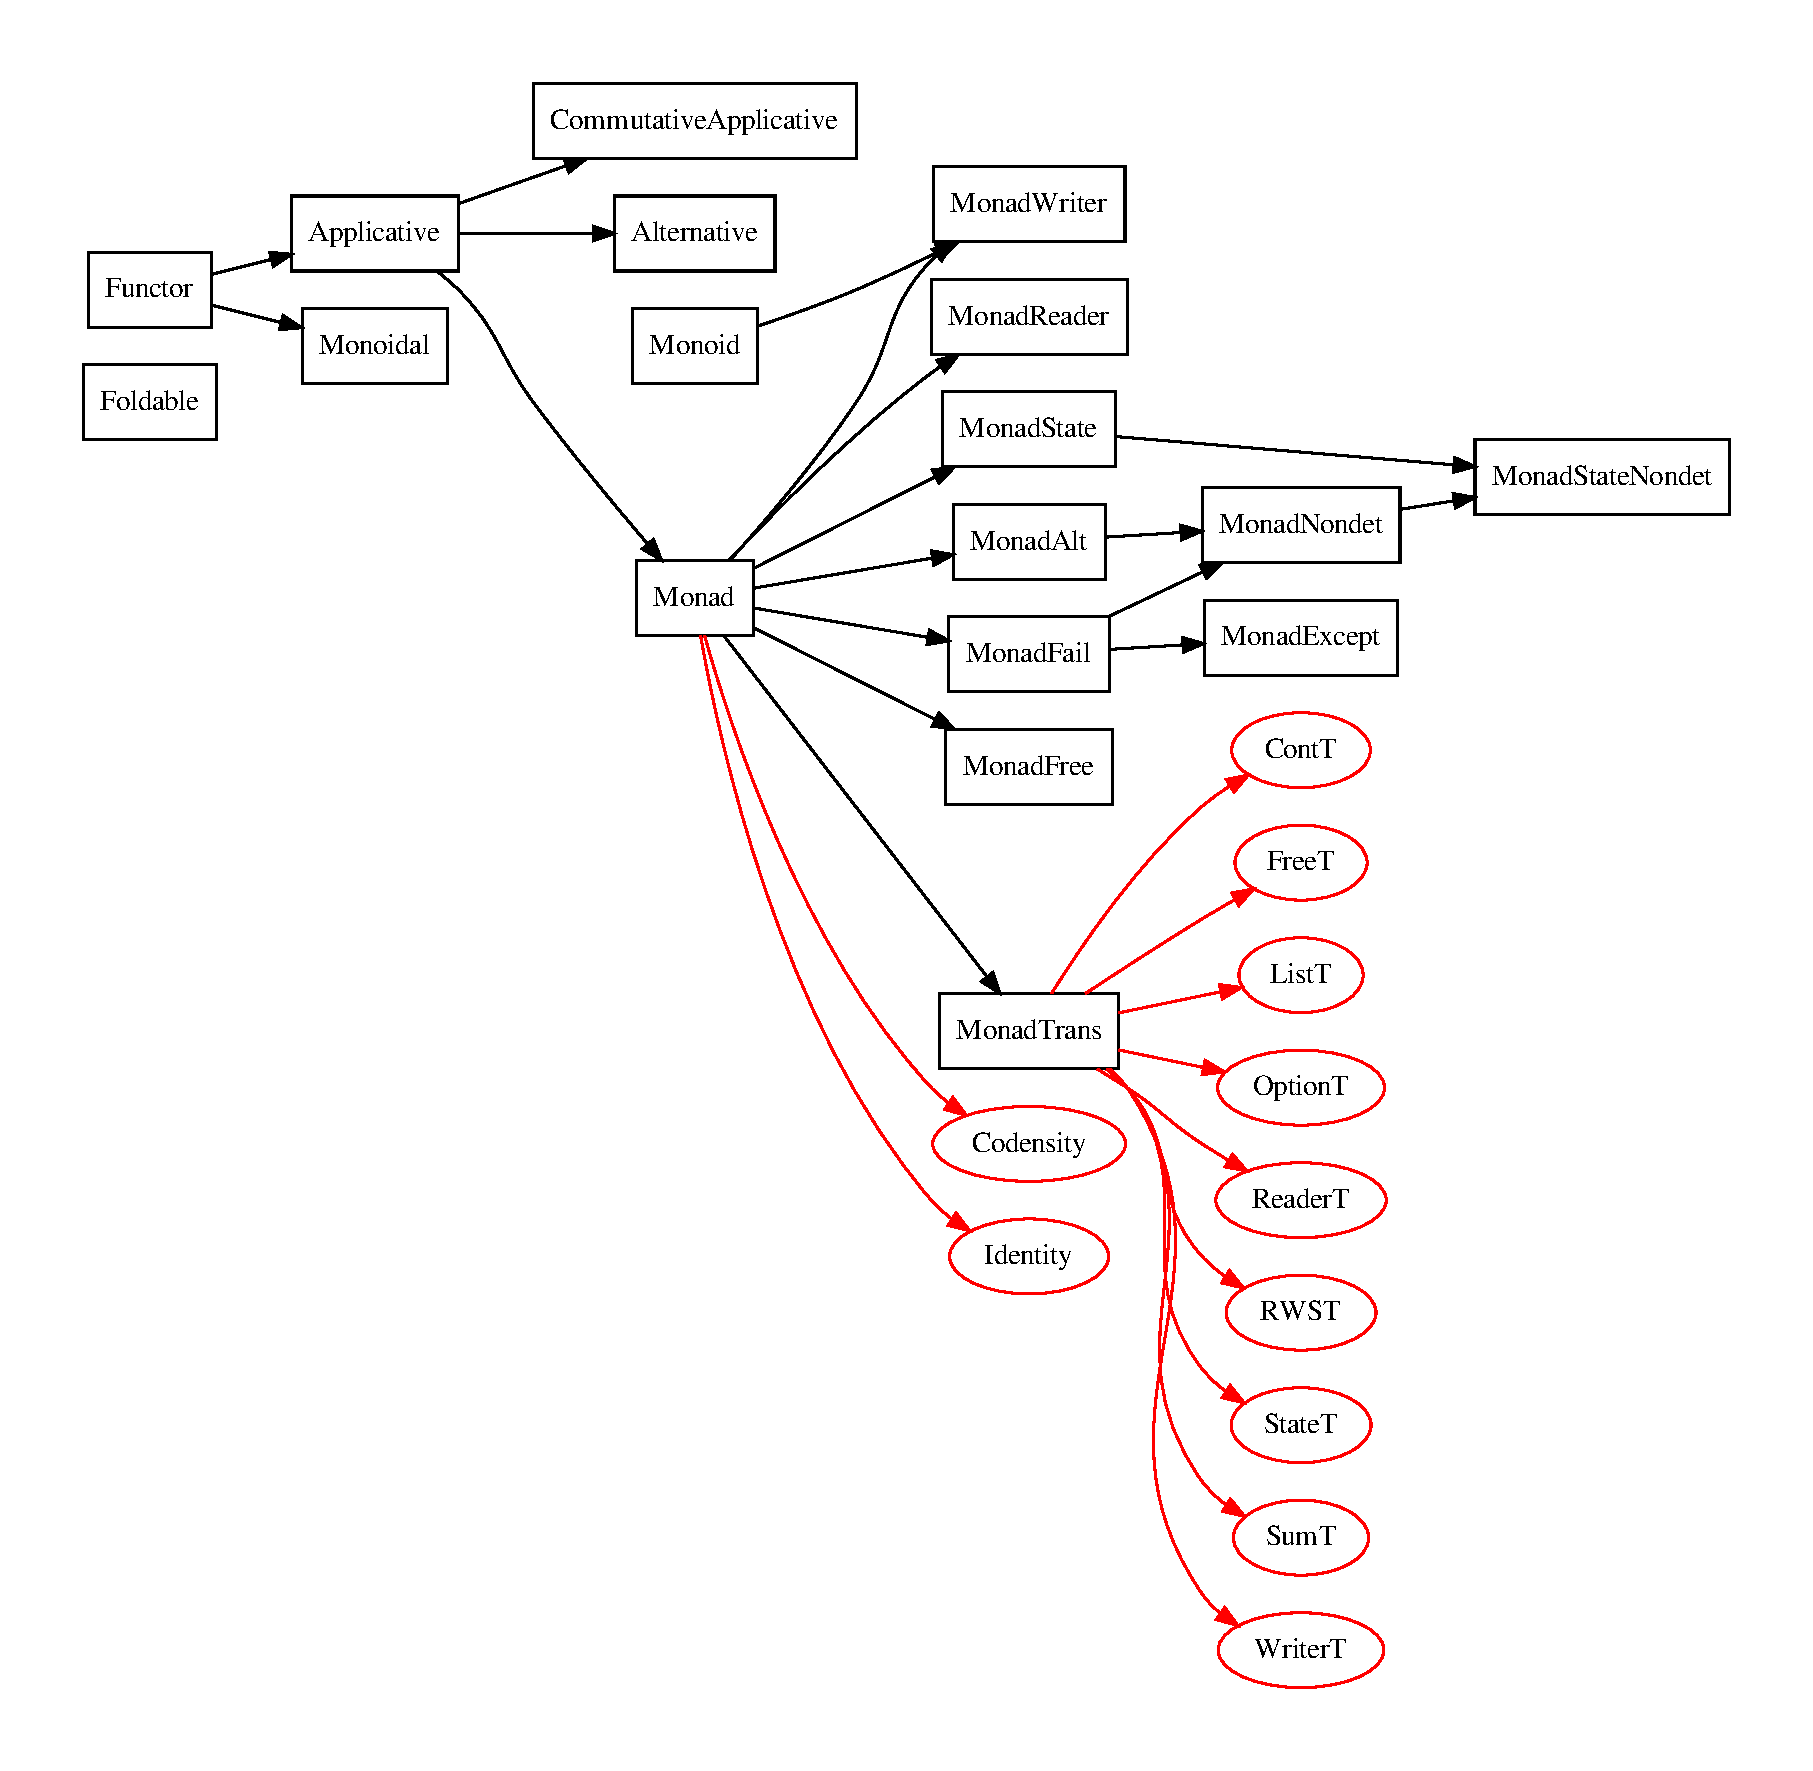
\includegraphics[width=20cm]{Hierarchy.pdf}}
    \caption{The library structure. Black boxes are classes, a black arrow from A to B means that class B depends on class A. Red ovals are class instances and a red arrow from A to B means that B is an instance of class A. A few classes were omitted (mainly variants of \m{MonadAlt}) and instances of the monadic effect classes (\m{MonadWriter} through \m{MonadFree}) were also omitted, as they would make the diagram unreadable.}
    \label{fig:hierarchy}
\end{figure}

\subsection{Typeclasses, canonical structures and modules}

The good news is that Coq has various mechanisms for achieving abstraction and modularity, such as typeclasses, canonical structures \cite{CanonicalStructures1} \cite{CanonicalStructures2} \cite{CanonicalStructures3} and modules \cite{Modules1} \cite{Modules2}. The bad news is that these mechanisms are related, overlapping, and their use inside the standard library and in third party libraries is not very consistent. We will therefore try to explain the similarities and differences motivating our choice of using classes to implement the library.

Typeclasses \cite{Classes1} \cite{Classes2} were originally invented for the purpose of overloading arithmetical operators in Haskell, but since then they were found to have many more applications and spread to other languages, like Rust.

In Coq, typeclasses are basically parametrized dependent records (collections of fields where types of later fields can depend on values of earlier fields and all of the fields can depend on the parameters) together with the mechanism of instance search (implemented using ordinary proof search) and a priority mechanism for deciding between overlapping instances.

In comparison to Haskell's, Coq's typeclasses are more powerful, as they are both first-class and higher-order. For example, in Coq we can have functions which take functions between typeclasses as inputs and return functions between typeclasses as outputs. Such constructions are not allowed in Haskell.

Canonical structures are a mechanism unique to Coq. They were introduced in a 1998 French PhD thesis \cite{CanonicalStructures0} and remain quite obscure since then, but see \cite{CanonicalStructures1} \cite{CanonicalStructures2} \cite{CanonicalStructures3}. They are built on the foundation of parametrized dependent records, just like typeclasses, but they differ from the latter in the instance search mechanism -- canonical structures are found using unification and not ad hoc proof search.

They also lack native handling of overlapping instances and backtracking, but this can be remedied with some hacks (see the conclusion section of \cite{CanonicalStructures2} for a detailed comparison). They are usually coupled with the module mechanism -- this approach is well present in the Mathematical Components library \cite{MCB}, a spin-off of the formalizations of the Four Colour Theorem. \cite{FourColour1} \cite{FourColour2}

The last of Coq's abstraction mechanisms is the module system \cite{Modules1} \cite{Modules2}, inspired by the module system of ML. A module, just like typeclasses and canonical structures, are very similar to parametrized dependent records (though not implemented using them), but they are less restrictive, because the body of a module can also contain vernacular commands, like inductive type definitions.

It is precisely these inductive type definitions that forbid Coq modules from being first-class (it may come as a surprise, but defining a new type can be considered an effect, because new named constants are added into the environment). Modules are also often used as namespaces, because all names declared in a module must be accessed by prefixing them with the module name, unless the module is imported into scope.

Our abstraction and modularity mechanism of choice were typeclasses. The most important reason was that we wanted the library to be intelligible to people with Haskell background, so all the basic design choices (not only the uses of classes, but also the whole class hierarchy up to monad transformers, naming of modules and functions, etc.) were made to match Haskell. An additional motivation was that the only other work on monads in Coq \cite{MERC} uses canonical structures. Together with the monadic effect classes taken from \cite{JustDoIt}, this results in the hierarchy of classes and their instances shown in figure \ref{fig:hierarchy}.

\subsection{Telescopes, setoids and other exotic animals}

\subsection{Axioms}

A very important property of every Coq development is being axiom free. The main reason is that the computational content of type theory is very axiom-sensitive. Because every axiom is just an element of some type, postulating it breaks the important property of canonicity. For example, if we postulate an axiom \m{nimber} of type \m{nat}, how does the term \m{nimber + 42} evaluate? The answer is that we don't know (or rather, it doesn't), because the definition of addition only handles the cases of zero and successor. This term is therefore stuck, i.e. it ``doesn't compute''.

\libname\ doesn't have this property. This is because a lot of monad laws (and other laws too), to be proved, require the functional extensionality axiom, which states that two functions are equal as soon as they have equal results for all inputs. We therefore adopt this axiom from the very beginning and use it wherever we need it without explicit mention. The resulting loss of canonicity isn't that bad, however, because it only prevents us from performing some computations with equality proofs, which are not at all important. We therefore consider adopting this axiom to be justified.

\section{Implementation}

1. Functor, Applicative, Monad.

2. Applicative-monad proposal etc.

3. Laws and minimal sets of laws.

\subsection{Proofs}

why no ssreflect? Ltac vs reflection. A case study in proof engineering - how do the tactics hs, monad work.

4. Transformers.

5. Classes from JustDoIt. Improvements over mtl.

\chapter{Examples, theorems and proofs}

1. Reasoning with concrete monads: rewrite example from chapter 1.

2. Reasoning with classes: towers of hanoi, fast product, JustDoIt.

3. Some theorems and proofs:

3.1. Laws for monad not minimal.

3.2. Applicative is Monoidal.

3.3. Equivalence of Monad definitions.

\chapter{Conclusion}

We have introduced \libname, a general purpose Coq library for formally verified programming with Haskell-style abstractions. We have centered our presentation on the matter effects, with which we dealt by implementing a collection of \m{mtl}-like abstractions whose main inspiration was \cite{JustDoIt}.

In chapter 1 we gave some arguments for why formal verification is worth pursuing and introduced the Coq proof assistant. In chapter 2 we explained the basics of computational effects and outlined the main approaches. In chapter 3 we elucidated the design choices, which weren't really that many, described the implementation and explained the mechanism behind our proof automation. In chapter 4, we have formalized some examples from \cite{JustDoIt} to show the viability of the library. We also saw some simple theorems which prove our implementation correct, but are also useful from a practical point of view.

\section{Technical details}

The source code and build instructions for \libname\ and the source code of this thesis can be found at \homepage. The code is extensively commented and this is the only available kind of documentation. Pull requests and suggestions are welcome.

\section{Related work}

There has been relatively little work on effects in Coq. \cite{MERC} is another attempt at an \m{mtl}-like library for Coq. It is similar to our work by also drawing inspiration from \cite{JustDoIt}, but differs in technical details (it uses canonical structures instead of classes) and focus (their motivation is formalization of programming languages).

There is an implementation of effects in Coq, available at \cite{CoqIO}, that allows one to define programs with IO and even concurrency and then extract the code to OCaml. This development is, however, rather obscure (there is not even a single paper about it). There also is an implementation of exceptions by means of a translation from the Calculus of Constructions to itself, realized in Coq as a plugin \cite{FailureIsNotAnOption}.

Besides, there has been some work on formally verifying programs with algebraic effects and handlers in Coq \cite{CoqEff1} \cite{CoqEff2} and more generally, on effectful programming in Coq \cite{CoqEff3}.

Among dependently typed languages most similar to Coq, there has been some work on an effect system for Idris \cite{IdrisEffects}. Another languages that mixes dependent types and effects (and also refinement types) is F* \cite{FStar}.

\section{Further work}

There's still some work to be done. The TODO list can be found by looking at the \m{TODO} section in \m{README.md} and by searching the source code for the keywords \m{Abort}, \m{Admitted} and for the marker TODO.

First off, some proofs and instances are missing. For example, I could neither define an instance of \m{MonadExcept} for \m{FreeT} nor prove that none exists. The same is true for a few more transformer/class pairs.

Notations could get some love too. The current do notation requires the ugly \m{;;} for computations that don't bind their result and I couldn't even define the idiom brackets of Idris using Coq's notation mechanism.

Some more theoretical work would be to formally characterize the minimal sets of laws for the various classes and some more practical work would be to implement other useful abstractions known from Haskell, like \m{Traversable} and \m{Foldable}.

Another possibility is to rewrite the whole automation engine, so as to use proof by reflection \cite{CPDT}, which is more reliable than the more ad hoc tactics written in Ltac. The first step toward this goal has already been made with the tactic \m{reflect\_functor}, which implements basic principles of reasoning with functors.

Last but not least, as already mentioned, \libname\ is a great basis on which a library similar to Haskell's \m{extensible-effects} may be implemented.

%%%%% BIBLIOGRAFIA

\begin{thebibliography}{1}

    \bibitem{JustDoIt}
        Jeremy Gibbons and Ralf Hinze, \\
        \textit{Just do It: Simple Monadic Equational Reasoning}, 2011 \\
        \url{http://www.cs.ox.ac.uk/jeremy.gibbons/publications/mr.pdf}

    \bibitem{Meltdown}
        Moritz Lipp, Michael Schwarz, Daniel Gruss, Thomas Prescher, Werner Haas, Anders Fogh, Jann Horn, Stefan Mangard, Paul Kocher, Daniel Genkin, Yuval Yarom and Mike Hamburg, \\
        \textit{Meltdown: Reading Kernel Memory from User Space}, 2018 \\
        \url{https://meltdownattack.com/meltdown.pdf}

    \bibitem{Spectre}
        Paul Kocher, Jann Horn, Anders Fogh, Daniel Genkin, Daniel Gruss, Werner Haas, Mike Hamburg, Moritz Lipp, Stefan Mangard, Thomas Prescher, Michael Schwarz and Yuval Yarom, \\
        \textit{Spectre Attacks: Exploiting Speculative Execution}, 2019 \\
        \url{https://spectreattack.com/spectre.pdf}
    
    \bibitem{Heartbleed}
        \url{https://heartbleed.com},
        2019

    \bibitem{DeepSpec}
        \url{https://deepspec.org},
        2019

    \bibitem{Boeing}
        Gregory Travis, \\
        How the Boeing 737 Max Disaster Looks to a Software Developer, \\
        \url{https://spectrum.ieee.org/aerospace/aviation/how-the-boeing-737-max-disaster-looks-to-a-software-developer}
    
    \bibitem{FourColour1}
        Georges Gonthier,
        \textit{A computer-checked proof of the Four Colour Theorem}, 2005 \\
        \url{https://www.cl.cam.ac.uk/~lp15/Pages/4colproof.pdf}
    
    \bibitem{FourColour2}
        Georges Gonthier,
        \textit{Formal Proof -- The Four-Color Theorem}, 2008, \\
        \url{http://www.ams.org/notices/200811/tx081101382p.pdf}

    \bibitem{UnivalentFoundations}
        Vladimir Voevodsky,
        \textit{UNIVALENT FOUNDATIONS},
        slides for a talk given at IAS on 26 March 2014, \\
        \url{http://www.math.ias.edu/~vladimir/Site3/Univalent_Foundations_files/2014_IAS.pdf}

    \bibitem{Coq}
        \url{https://coq.inria.fr/}

    \bibitem{CurryHoward}
        Morten Heine Sørensen, Paweł Urzyczyn, \\
        \textit{Lectures on the Curry-Howard Isomorphism}, 2006
    
    \bibitem{SoftwareFoundations}
        Benjamin C. Pierce, Andrew W. Appel and many others, \\
        \textit{Software Foundations}, 2019, \\
        \url{https://softwarefoundations.cis.upenn.edu/}
    
    \bibitem{CoqArt}
        Yves Bertot and Pierre Castéran, \\
        \textit{Interactive Theorem Proving and Program Development \\ Coq'Art: The Calculus of Inductive Constructions}, 2004, \\
        \url{https://www.labri.fr/perso/casteran/CoqArt/}

    \bibitem{CPDT}
        Adam Chlipala,
        \textit{Certified Programming with Dependent Types}, 2019,
        \url{http://adam.chlipala.net/cpdt/}

    \bibitem{BillionDollarMistake}
        Tony Hoare,
        \textit{Null References: The Billion Dollar Mistake}, \\
        \url{https://www.infoq.com/presentations/Null-References-The-Billion-Dollar-Mistake-Tony-Hoare/}
    
    \bibitem{CWM}
        Saunders Mac Lane,
        \textit{Categories for the Working Mathematician}

    \bibitem{MonadTutorialFallacy}
        Brent Yorgey, \textit{Abstraction, intuition, and the ``monad tutorial fallacy''}, \\
        \url{https://byorgey.wordpress.com/2009/01/12/abstraction-intuition-and-the-monad-tutorial-fallacy/}

    \bibitem{Moggi}
        Eugenio Moggi, \textit{Notions of computation and monads}, \\
        \url{https://person.dibris.unige.it/moggi-eugenio/ftp/ic91.pdf}

    \bibitem{mtl}
        Mark P. Jones,
        \textit{Functional Programming with Overloading and Higher-Order Polymorphism}, \\
        \url{http://web.cecs.pdx.edu/~mpj/pubs/springschool95.pdf}

    \bibitem{ExtensibleEffects}
        Oleg Kiselyov, Amr Sabry, Cameron Swords, \\
        \textit{Extensible Effects. An Alternative to Monad Transformers}, \\
        \url{http://okmij.org/ftp/Haskell/extensible/exteff.pdf}

    \bibitem{Freer}
        Oleg Kiselyov, Hiromi Ishii, \\
        \textit{Freer Monads, More Extensible Effects}, \\
        \url{http://okmij.org/ftp/Haskell/extensible/more.pdf}

    \bibitem{Koka}
        Daan Leijen,
        \textit{Koka: Programming with Row Polymorphic Effect Types}, 2014, \\
        \url{https://www.microsoft.com/en-us/research/wp-content/uploads/2016/02/paper-20.pdf}

    \bibitem{Eff}
        \url{https://www.eff-lang.org/}

    \bibitem{Frank}
        Sam Lindley, Connor McBride, \textit{Do Be Do Be Do}, \\
        \url{http://homepages.inf.ed.ac.uk/slindley/papers/frankly-draft-march2014.pdf}

    \bibitem{MulticoreOCaml}
        \url{https://github.com/ocaml-multicore/ocaml-multicore}
        
    \bibitem{Helium}
        \url{https://bitbucket.org/pl-uwr/helium/src/master/}

    \bibitem{CoqIO}
        \url{https://coq.io}

    \bibitem{Agda}
        \url{https://github.com/agda/agda}

    \bibitem{Idris}
        \url{https://www.idris-lang.org/}

    \bibitem{MERC}
        Reynald Affeldt, David Nowak, \\
        \textit{Experimenting with Monadic EquationalReasoning in Coq} \\
        \url{http://jssst.or.jp/files/user/taikai/2018/PPL/ppl2-2.pdf}

    \bibitem{FailureIsNotAnOption}
        Pierre-Marie Pédrot, Nicolas Tabareau \\
        \textit{Failure is Not an Option: An Exceptional Type Theory}, \\
        \url{https://link.springer.com/chapter/10.1007/978-3-319-89884-1_9}

    \bibitem{CoqEff1}
        Jean-Guillaume Dumas, Dominique Duval, Burak Ekici, Damien Pous \\
        \textit{Formal verification in Coq of program properties involving the global state effect}, \\
        \url{https://hal.archives-ouvertes.fr/file/index/docid/872324/filename/DDEP-coqstates.pdf}

    \bibitem{CoqEff2}
        Thomas Letan, Yann Régis-Gianas, Pierre Chifflier, Guillaume Hiet, \\
        \textit{Modular Verification of Programs with Effects and Effect Handlers in Coq}, \\
        \url{https://hal.inria.fr/hal-01799712/document}

    \bibitem{CoqEff3}
        Greg Morrisett, \\
        \textit{Programming with Effects in Coq}, \\
        \url{https://link.springer.com/chapter/10.1007%2F978-3-540-70594-9_3}

    \bibitem{IdrisEffects}
        Edwin C. Brady, \\
        \textit{Programming and Reasoning with Algebraic Effects and Dependent Types}, \\
        \url{https://eb.host.cs.st-andrews.ac.uk/drafts/effects.pdf}

    \bibitem{FStar}
        \url{https://www.fstar-lang.org/}
    
    \bibitem{Classes1}
        Matthieu Sozeau, Nicolas Oury,
        \textit{First-Class Type Classes}, \\
        \url{https://www.irif.fr/~sozeau/research/publications/First-Class_Type_Classes.pdf}

    \bibitem{Classes2}
        \url{https://coq.inria.fr/distrib/current/refman/addendum/type-classes.html}

    \bibitem{CanonicalStructures0}
        Amokrane Saïbi, \\
        \textit{Outils Génériques de Modélisation et de Démonstration pour la Formalisation des Mathématiques en Théorie des Types. Application à la Théorie des Catégories.}, 1998, \\
        \url{https://tel.archives-ouvertes.fr/tel-00523810/file/Saibi_-_1999_-_Outils_GA_nA_riques_de_modA_lisation_et_de_dA_monstration_pour_la_Formalisation_des_MathA_matiques_en_thA_orie_des_Types_Application_A_la_thA_orie_des_catA_gories.pdf}

    \bibitem{CanonicalStructures1}
        Georges Gonthier, Beta Ziliani, Aleksandar Nanevski, Derek Dreyer, \\
        \textit{How to make ad hoc proof automationless ad hoc}, \\
        \url{https://software.imdea.org/~aleks/papers/lessadhoc/journal.pdf}

    \bibitem{CanonicalStructures2}
        Assia Mahboubi, Enrico Tassi, \\
        \textit{Canonical Structures for the working Coq user} \\
        \url{https://hal.inria.fr/hal-00816703v2/document}

    \bibitem{CanonicalStructures3}
        \url{https://coq.inria.fr/refman/addendum/canonical-structures.html}

    \bibitem{MCB}
        Assia Mahboubi and Enrico Tassi with contributions by Yves Bertot and Georges Gonthier, \\
        \url{https://math-comp.github.io/mcb/}

    \bibitem{Modules1}
        Jacek Chrząszcz,
        \textit{Modules in Coq Are and Will Be Correct}, \\
        \url{https://link.springer.com/chapter/10.1007%2F978-3-540-24849-1_9}

    \bibitem{Modules2}
        \url{https://coq.inria.fr/distrib/current/refman/language/module-system.html}
\end{thebibliography}

%\begin{thebibliography}{1}
%\bibitem{example} \ldots
%\end{thebibliography}

\end{document}